\documentclass[10pt, a4paper]{article}
\usepackage[utf8]{inputenc}
\usepackage[T1]{fontenc}
\usepackage[ngerman]{babel}
\usepackage{graphicx}
\usepackage{multicol}
\usepackage[left=1.5cm, right=1.5cm, top=2.5cm, bottom=2.5cm]{geometry}

% Verhindert das Einrücken neuer Absätze für eine saubere Darstellung der Listen
\setlength{\parindent}{0pt}
\setlength{\parskip}{0.5em}

\begin{document}

% --- TITELBLATT ---
\begin{titlepage}
    \centering
    \vspace*{5cm}
    {\Huge \textbf{Dokumentation Struktur und Beziehungen im CLD}\par}
    \vspace{2cm}
    {\Large Dokumentation pro Beziehung und Loop\par}
    \vfill
\end{titlepage}

% --- SEITE 2: HAUPTTITEL UND BILD ---
\section*{\centering Dokumentation Struktur und Beziehungen im CLD}

\vspace{1cm}
\begin{figure}[htbp]
    \centering
    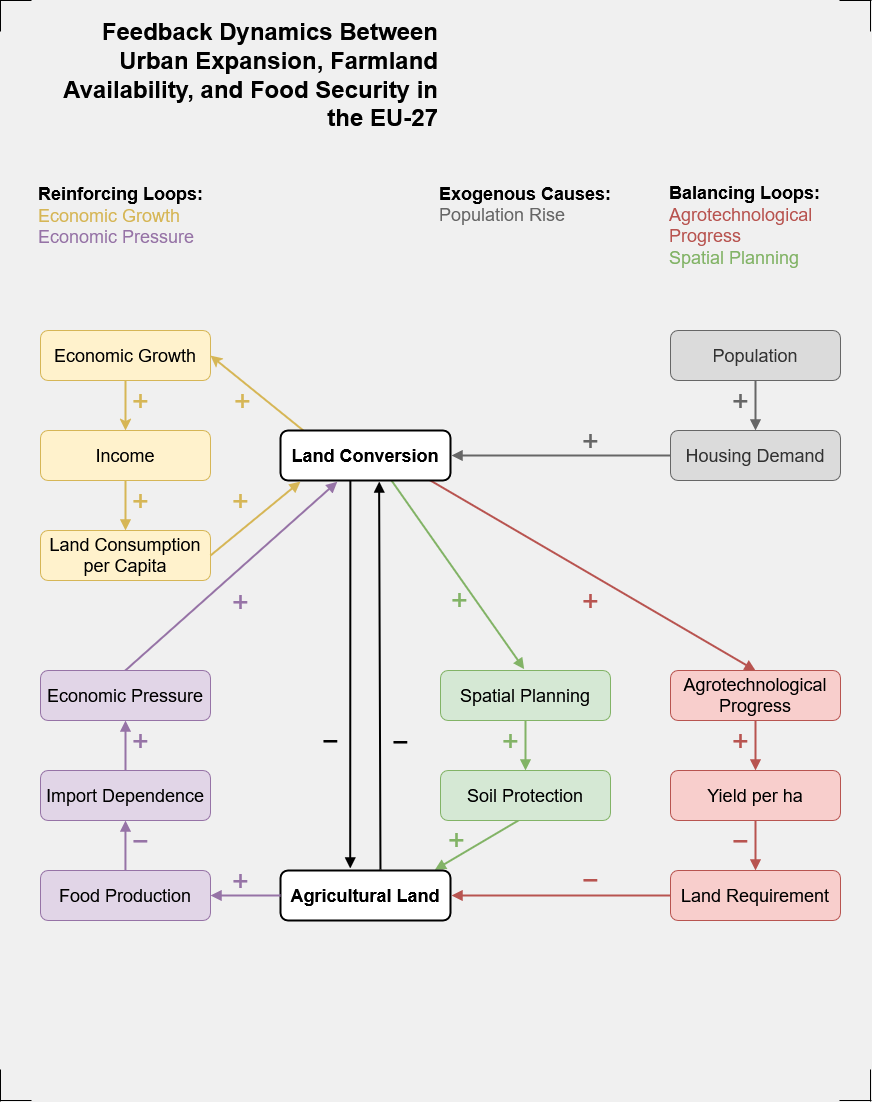
\includegraphics[width=0.8\textwidth]{./assets/cld.png}    
    \caption{Struktur und Beziehungen im CLD}
\end{figure}

\newpage

% --- HAUPTDOKUMENT ---
\small

\section*{\centering Dokumentation pro Beziehung im CLD}
\vspace{0.5cm}

% --- SEITE 3 (4 Beschreibungen) ---
\begin{multicols}{2}

% --- Spalte Links ---
\subsection*{Economic Growth $\rightarrow$ Income}
Wirtschaftliches Wachstum erhöht das durchschnittliche Einkommensniveau in einer Volkswirtschaft. 

\textbf{Wirkungslogik:}\\
Die Beziehung wird zunächst als annähernd linear modelliert. Keine expliziten Schwellenwerte oder Sättigungen werden modelliert.

\textbf{Vorzeichen:} +

\textbf{Zeit:}\\
Die Wirkung erfolgt mit kurz- bis mittelfristiger Verzögerung, da Einkommensveränderungen über Arbeitsmarkt- und Produktivitätsdynamiken entstehen.

\textbf{Annahmen:}\\
Wirtschaftswachstum wirkt positiv auf Einkommen.\\
Verteilungsfragen werden nicht modelliert.

\textbf{Evidenzbasis:}\\
Theoretisch begründet (makroökonomischer Standardmechanismus).

\textbf{Unsicherheitsgrad:}\\
Niedrig

\vspace{0.5cm} % Abstand zur zweiten Beschreibung in derselben Spalte

\subsection*{Income $\rightarrow$ Land Consumption per Capita}
Steigendes Einkommen erhöht tendenziell den Flächenverbrauch pro Person, z.B. durch grössere Wohnflächen, suburbanes Wohnen oder Infrastruktur.

\textbf{Wirkungslogik:}\\
Die Wirkung wird als indirekte sozioökonomische Beziehung verstanden.

Die Beziehung wird als monoton steigend modelliert.

\textbf{Vorzeichen:} +

\textbf{Zeit:}\\
Verzögerung durch Bauprozesse, Infrastrukturentwicklung und Haushaltsentscheidungen.

\textbf{Annahmen:}\\
Höheres Einkommen führt im Durchschnitt zu höherem Flächenkonsum.

\textbf{Evidenzbasis:}\\
Empirisch gestützt durch Urban-Sprawl-Literatur.

\textbf{Unsicherheitsgrad:}\\
Mittel

\vfill\columnbreak % Zwingt den restlichen Text in die rechte Spalte

% --- Spalte Rechts ---
\subsection*{Land Consumption per Capita $\rightarrow$ Land Conversion}
Steigender Flächenverbrauch pro Person erhöht den Bedarf an zusätzlicher Siedlungsfläche und führt zur Umwandlung landwirtschaftlicher Flächen.

\textbf{Wirkungslogik:}\\
Die Beziehung wird als monoton steigend modelliert.

\textbf{Vorzeichen:} +

\textbf{Zeit:}\\
Strukturelle Verzögerung durch Planungs- und Bauprozesse.

\textbf{Annahmen:}\\
Verdichtungsstrategien kompensieren den Effekt nicht vollständig.

\textbf{Evidenzbasis:}\\
Empirisch dokumentiert (EU Land Take Studien).

\textbf{Unsicherheitsgrad:}\\
Mittel

\vspace{0.5cm}

\subsection*{Land Conversion $\rightarrow$ Agricultural Land}
Die Umwandlung von Land in Siedlungsfläche reduziert direkt die verfügbare landwirtschaftliche Fläche. 

\textbf{Wirkungslogik:}\\
Agricultural Land wird als Bestandsvariable modelliert, deren Umfang durch Flächenumwandlungen reduziert wird.

Die Beziehung wird als monoton steigend modelliert.

\textbf{Vorzeichen:} --

\textbf{Zeit:}\\
Direkte Wirkung nach Umsetzung der Landnutzungsänderung.

\textbf{Annahmen:}\\
Rückumwandlung (Renaturierung) ist strukturell nicht dominant.

\textbf{Evidenzbasis:}\\
Empirisch gut dokumentiert.

\textbf{Unsicherheitsgrad:}\\
Niedrig

\end{multicols}
\newpage

% --- SEITE 4 (4 Beschreibungen) ---
\begin{multicols}{2}

% --- Spalte Links ---
\subsection*{Agricultural Land $\rightarrow$ Food Production}
Mehr landwirtschaftliche Fläche erhöht bei konstantem Ertrag die mögliche Nahrungsmittelproduktion.

\textbf{Wirkungslogik:}\\
Food Production wird als Funktion der landwirtschaftlichen Fläche und des Flächenertrags modelliert. \\
Die Beziehung wird als monoton steigend modelliert.

\textbf{Vorzeichen:} +

\textbf{Zeit:}\\
Produktionsverzögerung durch landwirtschaftliche Zyklen.

\textbf{Annahmen:}\\
Produktion proportional zur Fläche bei gegebenem Ertrag.

\textbf{Evidenzbasis:}\\
Agrarökonomische Standardbeziehung.

\textbf{Unsicherheitsgrad:}\\
Niedrig

\vspace{0.5cm}

\subsection*{Agrotechnological Progress $\rightarrow$ Yield per ha}
Technologischer Fortschritt erhöht die Produktivität pro Flächeneinheit.

\textbf{Wirkungslogik:}\\
Die Beziehung wird als monoton steigend modelliert.

\textbf{Vorzeichen:} +

\textbf{Zeit:}\\
Langsame Diffusion von Innovationen.

\textbf{Annahmen:}\\
Fortschritt wirkt überwiegend positiv auf Erträge.

\textbf{Evidenzbasis:}\\
Empirisch gut dokumentiert.

\textbf{Unsicherheitsgrad:}\\
Mittel

\vfill\columnbreak

% --- Spalte Rechts ---
\subsection*{Yield per ha $\rightarrow$ Food Production}
Steigende Erträge erhöhen bei gleicher Fläche die Gesamtproduktion.

\textbf{Wirkungslogik:}\\
Yield per ha bestimmt gemeinsam mit der landwirtschaftlichen Fläche die Produktionsmenge.\\
Die Beziehung wird als monoton steigend modelliert.

\textbf{Vorzeichen:} +

\textbf{Zeit:}\\
Wirkung tritt mit landwirtschaftlichen Produktionszyklen ein.

\textbf{Annahmen:}\\
Keine starke Ertragsdegradation berücksichtigt.

\textbf{Evidenzbasis:}\\
Empirisch belegt.

\textbf{Unsicherheitsgrad:}\\
Niedrig

\vspace{0.5cm}

\subsection*{Food Production $\rightarrow$ Import Dependence}
Sinkende heimische Nahrungsmittelproduktion erhöht die Abhängigkeit von Importen.

\textbf{Wirkungslogik:}\\
Import Dependence wird als Funktion der Differenz zwischen inländischer Produktion und Nachfrage interpretiert.

\textbf{Vorzeichen:} --

\textbf{Zeit:}\\
Kurzfristige Anpassung über Handelsmärkte.

\textbf{Annahmen:}\\
Die EU ist kein vollständig autarkes Ernährungssystem.

\textbf{Evidenzbasis:}\\
Handelsökonomisch plausibel.

\textbf{Unsicherheitsgrad:}\\
Mittel

\end{multicols}
\newpage

% --- SEITE 5 (Restliche 2 Beschreibungen) ---
\begin{multicols}{2}

% --- Spalte Links ---
\subsection*{Import Dependence $\rightarrow$ Economic Pressure}
Steigende Importabhängigkeit erzeugt wirtschaftlichen Druck. Import Dependence wird im Modell als Indikator für Versorgungssicherheit interpretiert.

\textbf{Wirkungslogik:}\\
Steigende Importabhängigkeit kann wirtschaftlichen oder politischen Druck erzeugen, die heimische Produktion oder wirtschaftliche Aktivität zu steigern.\\
Die Beziehung wird als monoton steigend modelliert.

\textbf{Vorzeichen:} +

\textbf{Zeit:}\\
Mittelfristige politische und wirtschaftliche Anpassungsprozesse.

\textbf{Annahmen:}\\
Importabhängigkeit wird politisch und ökonomisch als Problem wahrgenommen.

\textbf{Evidenzbasis:}\\
Teilweise theoretisch, teilweise hypothesenbasiert.

\textbf{Unsicherheitsgrad:}\\
Hoch

\vfill\columnbreak

% --- Spalte Rechts ---
\subsection*{Economic Pressure $\rightarrow$ Land Conversion}
Wirtschaftlicher Druck stärkt die wirtschaftliche Ausrichtung der Nutzung von Flächen .

\textbf{Wirkungslogik:}\\
Die Beziehung wird als monoton steigend modelliert.

\textbf{Vorzeichen:} +

\textbf{Zeit:}\\
Politisch-institutionelle Verzögerung.

\textbf{Annahmen:}\\
Wirtschaftliche Nutzung konkurriert mit Flächenschutzinteressen.

\textbf{Evidenzbasis:}\\
Explorative Annahme.

\textbf{Unsicherheitsgrad:}\\
Hoch

\end{multicols}
\newpage

% --- SEITE 6: LOOP KAPITEL (4 Beschreibungen) ---
\section*{\centering Dokumentation pro Loop}
\vspace{0.5cm}

\begin{multicols}{2}

% --- Spalte Links ---
\subsection*{R1 – Import Pressure Loop}
Sinkende Produktion aufgrund von Land Conversion produziert Importabhängigkeit. Daraus resultierender ökonomischer Druck fördert Land Conversion.

Land Conversion $\rightarrow$ Agricultural Land $\rightarrow$ Food Production $\rightarrow$ Import Dependence $\rightarrow$ Economic Pressure $\rightarrow$ Land Conversion

\textbf{Typ:} Reinforcing

\textbf{Dominanzannahme:}\\
Relevant bei hoher Marktintegration.

\vspace{0.5cm}

\subsection*{R2 – Economic Growth Loop (Gelb)}
Land Conversion fördert wirtschaftliches Wachstum, was die  Flächennachfrage erhöht, was zu erhöhter Land Conversion führt.

Economic Growth $\rightarrow$ Income $\rightarrow$ Land Consumption per Capita $\rightarrow$ Land Conversion $\rightarrow$ Economic Growth

\textbf{Typ:} Reinforcing

\textbf{Dominanzannahme:}\\
Dominant bei wachstumsorientierten politischen Rahmenbedingungen.

\vfill\columnbreak

% --- Spalte Rechts ---
\subsection*{B1 – Agricultural Technology Loop}
Agrotechnologischer Fortschritt kann die Produktivität per Hektar landwirtschaftlicher Fläche erhöhen, was bei gleichbleibender Nahrungsmittelproduktion den Bedarf an landwirschafflicher Totalfläche  reduziert.

Land Conversion $\rightarrow$ Agrotechnological Progress $\rightarrow$ Yield per ha $\rightarrow$ Land Requirement $\rightarrow$ Agricultural Land $\rightarrow$ Land Conversion 

\textbf{Typ:} Balancing

\textbf{Dominanzannahme:}\\
Wirksam bei starkem technologischen Fortschritt.

\vspace{0.5cm}

\subsection*{B2 – Spatial Planning Loop}
Abnehmende Landwirtschaftsfläche kann politisch problematisiert werden. Darauf folgende Raumplanung stabilisiert über regulatorische Massnahmen die landwirtschaftliche Fläche, was wiederum die Land Conversion abbremst

Land Conversion $\rightarrow$ Spatial Planning $\rightarrow$ Soil Protection $\rightarrow$ Agricultural Land $\rightarrow$ Land Conversion

\textbf{Typ:} Balancing

\textbf{Dominanzannahme:}\\
Abhängig von institutioneller Stärke.

\end{multicols}

\end{document}
